\documentclass[main.tex]{subfiles}
\begin{document}
\chapter{Mechanics}
\section{Scalars and Vectors}
\spec{(a) distinguish between scalar and vector quantities and give examples of each}
A scalar quantity\footnote{strictly we are modelling a physical quantity as a mathematical object} is one which has only a magnitude whereas a vector has \emph{both} magnitude and direction. We often use positive and negative values to indicate direction (e.g. $v=-2\ ms^{-1}$) but this does not mean that all negative values are vectors!

Note that there are different ways of multiplying vectors and scalars. Two vectors can be multiplied to give a scalar \emph{or} a vector. For example, word done is the (scalar) product of force and displacement, both vectors.

\spec{(b) resolve a vector into two components at right angles to each other by drawing and by calculation}

Vectors can be split into two components using trigonometry. The diagram below shows a velocity vector being split into horizontal and vertical components $v_x$ and $v_y$.

\begin{center}
\begin{tikzpicture}
	\draw[very thick, black, ->] (0,0) -- node[above] {$\mathbf{v}$}  (5,2.5);
	\draw[very thick, red, ->] (0,0) -- node[below] {$\mathbf{v_x}$} (5,0);
	\draw[very thick, red, ->] (0,0) -- node[left]{$\mathbf{v_y}$}(0,2.5);
	\draw [very thick,gray](1,0) arc (0:26.6:1);
	\draw [gray](1,0.25) node[right]{$\theta$};
	\draw (7,1.25) node[right] {
		$\begin{aligned}
		\mathbf{v}&=\mathbf{v_x + v_y}\\
		v_x &= v\cos{\theta}\\
		v_y &= v\sin{\theta}
		\end{aligned}$};
\end{tikzpicture}
\end{center}

\spec{(c) combine any number of coplanar vectors at any angle to each other by drawing}

Vectors can be added by placing them end to end. The resultant vector is the one joining the start of the first vector to the end of the final vector. Its magnitude and direction can be calculated by trigonometry or scale drawing.

\begin{center}
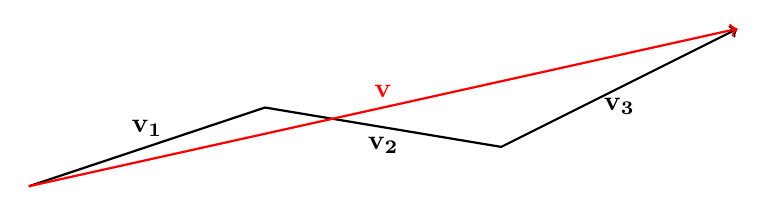
\begin{tikzpicture}
\draw[thick,->] (0,0) -- node[above] {$\mathbf{v_1}$} (3,1) -- node[below] {$\mathbf{v_2}$} (6,.5) -- node[below] {$\mathbf{v_3}$} (9,2);
\draw[thick,red,->] (0,0) -- node[above]{$\mathbf{v}$} (9,2);
\end{tikzpicture}
$$\mathbf{v} = \mathbf{v_1}+\mathbf{v_2}+\mathbf{v_3}$$
\end{center}

\section{Forces and Accelerations}

\spec{(d) calculate the moment of a force and use the conditions for equilibrium to solve problems (restricted to
	coplanar forces)}

\end{document}
